\documentclass[10pt,openright,twoside,french]{book}

\input philippe2013
\input philippe2013_cours
\input philippe2013_sections
\input philippe2013_chapitre

\pagestyle{empty}
\pieddepage{}{}{}

\setcounter{chapter}{7}
\begin{document}

\renewcommand\PartProgramme{Stats/Probas}
\chapter[Statistiques continues]{Statistiques continues\\ Analyse de données}\label{ch_statistiques_continues}

\section{Vocabulaire}

\begin{Defi}
    Dans une série statistique continue, un caractère continu quantitatif peut prendre toutes les valeurs d'un intervalle. On dit que les données sont regroupées par \ipt{classe}. L'\ipt{amplitude} de la classe est la longueur de l'intervalle.
\end{Defi}

\begin{Defi}
    On considère la classe $\intervallefo a b$ ou $\intervalleff a b$.\par
    On appelle \ipt{centre de classe} la moyenne des valeurs extrêmes : \[c = \frac{a + b}{2}.\]
\end{Defi}

\begin{Exemple}
    On note la répartition des salariés d'une entreprise suivant le salaire mensuel. Le salaire étant un caractère continu, on peut utiliser un regroupement par classe :
    \begin{center}
    \renewcommand\arraystretch{2}
        \begin{tabular}{|c|c|c|}
            \hline
                Tranches de salaires & Effectifs & Centre de classe \\
            \hline
                $\intervallefo{0}{250}$ & $10$ & $125$\\
            \hline
                $\intervallefo{250}{500}$ & $15$ & $375$\\
            \hline
                $\intervallefo{500}{750}$ & $45$ & $625$\\
            \hline
                $\intervallefo{750}{\np{1000}}$ & $110$ & $875$\\
            \hline
                $\intervallefo{\np{1000}}{\np{1250}}$ & $255$ & $\np{1125}$\\
            \hline
                $\intervallefo{\np{1250}}{\np{1500}}$ & $150$ & $\np{1375}$\\
            \hline
                $\intervallefo{\np{1500}}{\np{1750}}$ & $60$ & $\np{1625}$ \\
            \hline
                $\intervallefo{\np{1750}}{\np{2000}}$ & $35$ & $\np{1875}$ \\
            \hline
        \end{tabular}
    \renewcommand\arraystretch{1}
    \end{center}
\end{Exemple}

\begin{Rmq}
    Pour calculer la moyenne d'une série continue, on utilise les effectifs et les centres de classe :
    \[\overline m = \dfrac{10 \times 125 + \cdots + 35 \times \np{1875}}{10 + \cdots + 35}\]
\end{Rmq}\clearpage

\section{Fréquences cumulées croissantes}

\begin{Defi}
    La \ipt{fréquence} $f$ d'une valeur est donnée par la formule suivante : \[f = \frac{\text{effectif de la valeur}}{\text{effectif total}}.\]
\end{Defi}

\begin{Rmq}
    Une fréquence est toujours comprise entre $0$ et $1$.
\end{Rmq}

\begin{Defi}
    La \iptb{fréquence cumulée croissante}\index{fréquence!cumulée croissante} associée à une valeur $a$ est égale à la somme des fréquences de toutes les valeurs inférieures ou égales à $a$.
\end{Defi}

\begin{Exemple}
    \renewcommand\arraystretch{2.5}
        \begin{tabular}[t]{|c|c|c|}
            \hline
                Tranches de salaires & Fréquence & FCC \\
            \hline
                $\intervallefo{0}{250}$ & $\frac{10}{680} \approx 1,47\%$ & $1,47\%$\\
            \hline
                $\intervallefo{250}{500}$ & $2,21\%$ & $3,68\%$\\
            \hline
                $\intervallefo{500}{750}$ & $6,62\%$ & $10,29\%$\\
            \hline
                $\intervallefo{750}{\np{1000}}$ & $16,18\%$ & $26,47\%$\\
            \hline
                $\intervallefo{\np{1000}}{\np{1250}}$ & $37,5\%$ & $63,97\%$\\
            \hline
                $\intervallefo{\np{1250}}{\np{1500}}$ & $22,06\%\%$ & $86,03\%$\\
            \hline
                $\intervallefo{\np{1500}}{\np{1750}}$ & $8,82$ & $94,85\%$ \\
            \hline
                $\intervallefo{\np{1750}}{\np{2000}}$ & $5,15$ & $100\%$ \\
            \hline
        \end{tabular}
\end{Exemple}

\begin{center}
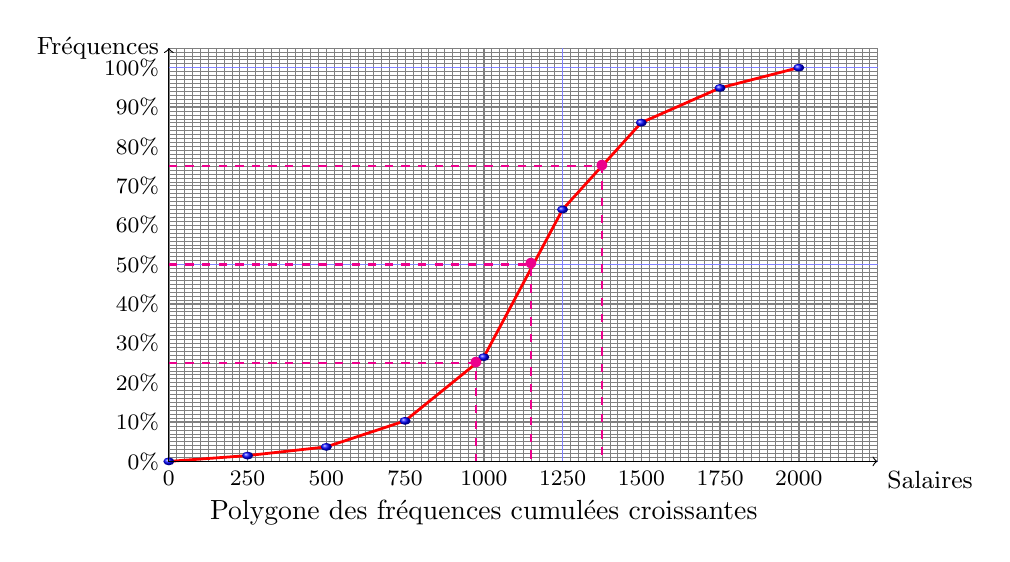
\begin{tikzpicture}[yscale=0.05]
	% Dimensions du repere
	\def\xmin{0} \def\xmax{9} \def\ymin{0} \def\ymax{105}
	% Grilles
	\draw [xstep=0.1,ystep=1,gray,very thin]  (\xmin,\ymin) grid (\xmax,\ymax);
	\draw [xstep=1,ystep=10,gray,thin] (\xmin,\ymin) grid (\xmax,\ymax);
	\draw [xstep=5,ystep=50,thin,color=blue!50]  (\xmin,\ymin) grid (\xmax,\ymax);
    \draw (4,-13) node {Polygone des fréquences cumulées croissantes};
    \draw[line width = 1pt,red] plot[mark=ball,mark options={yscale = 14.3}] coordinates{(0,0)(1,1.47)(2,3.68)(3,10.29)(4,26.47)(5,63.97)(6,86.03)(7,94.85)(8,100)};
    \draw[<->] (0,105) node[left] {\small Fréquences} -- (0,0) -- (9,0) node[below right] {\small Salaires};
    \foreach \x in {0,250,...,2000} \draw ({\x / 250},0) node[below] {\footnotesize $\x$};
    \foreach \x in {0,10,...,100} \draw (0,\x) node[left] {\footnotesize $\x\%$};
    \draw[magenta,dashed,line width=0.75pt] (0,50) -- (4.6,50) node {$\bullet$} -- (4.6,0);
    \draw[magenta,dashed,line width=0.75pt] (0,25) -- (3.9,25) node {$\bullet$} -- (3.9,0);
    \draw[magenta,dashed,line width=0.75pt] (0,75) -- (5.5,75) node {$\bullet$} -- (5.5,0);
\end{tikzpicture}
\end{center}

D'après le polygone des fréquences cumulées croissantes, on peut déterminer graphiquement une valeur des indicateurs de position :
\[\text{Médiane} \approx \np{1150} \qq Q_1 \approx 975 \qetq Q_3 \approx \np{1375}.\]

\section{Histogramme}

\begin{Defi}
Un \ipt{histogramme} est une représentation graphique d'une série statistique de variable quantitative.\par
Il est constitué de rectangles contigus dont les \textbf{aires sont proportionnelles aux effectifs} de chaque classe.\par
Sur l'axe des abscisses sont reportées les bornes des classes de la série.
\end{Defi}

\subsection{Histogramme à pas constant}

\subsection{Histogramme à pas non constant}

\begin{center}
\renewcommand\arraystretch{2}
\begin{tabular}{*{7}{|c}|}
\hline
    Salaire & $\intervallefo{900}{200}$ & $\intervallefo{1200}{1400}$ & $\intervallefo{1400}{1600}$ & $\intervallefo{1600}{1800}$ & $\intervallefo{1800}{2000}$ & $\intervalleff{2000}{2400}$ \\
\hline
    Effectif & 30 & 30 & 60 & 40 & 20 & 10 \\
\hline
\end{tabular}
\renewcommand\arraystretch{1}
\end{center}

\end{document} 